Here, we discuss the face code generation from numerical values of facial attributes. This is the most important and innovative module in our system and the first stage of \emph{face generation}. It's worth noting that we use both of the terms \emph{"feature"} and \emph{"attribute"} to refer to a facial attribute, like hair color or nose size.

\begin{figure}[H]
    \centering
    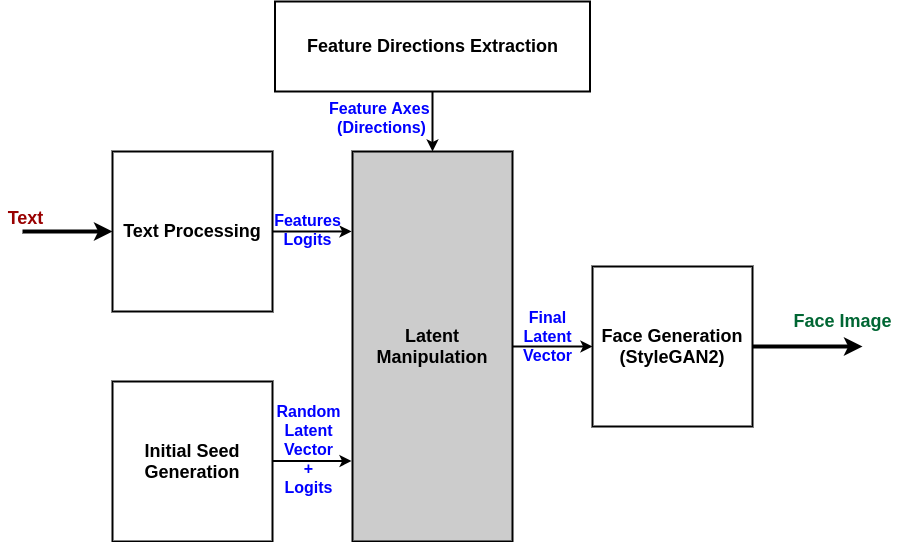
\includegraphics[width=0.8\textwidth]{images/face-gen-arch.png}
    \caption{Detailed block diagram of the three core modules workflow}
    \label{fig:face_gen}
\end{figure}

\subsubsection{Functional Description}

Figure \ref{fig:face_gen} shows a block diagram of the interaction between the $3$ core modules. We can see that the code generation module is the main driver of our face generation process. Generally, it converts the numerical attributes values (a.k.a. \emph{logits}) into a face embedding vector that matches the design of the latent space of the face generator (\emph{StyleGAN2}). Basically, it starts from an initial vector and uses the \emph{required feature values} and \emph{extracted feature directions} to transform this vector into the final latent vector, which is passed to the generative model.

\begin{itemize}
    \item \textbf{Input :}
    \begin{itemize}
        \item Numerical values of facial features (logits).
    \end{itemize}
    \item \textbf{Output :}
    \begin{itemize}
        \item Low dimensional face embedding vector (latent vector).
    \end{itemize}
\end{itemize}

\subsubsection{Modular Decomposition}

As figure \ref{fig:face_gen} tells, the code generation module can be torn down into $3$ sub-modules, which are \textbf{latent manipulation}, \textbf{initial seed generation} and \textbf{feature directions extraction}. Each sub-module is discussed in details to show how they integrate to each other to achieve the desired goal.

\paragraph{Feature Directions Generation}
Since, we use \texttt{StyleGAN2} \cite{karras2020analyzing} as our generative model, we have a full $512D$ latent space that is used to encode the whole face attributes. The changes in this latent space maps to the generated face image and similar features occupies the same area in the latent space. Consequently, we have to come up with a way to extract the axes (\emph{hyperplanes}) in this latent space to define each of our $32$ facial features. These feature directions are, then, used to manipulate the latent vector, in order to map to the required face image. 

\begin{figure}[H]
    \centering
    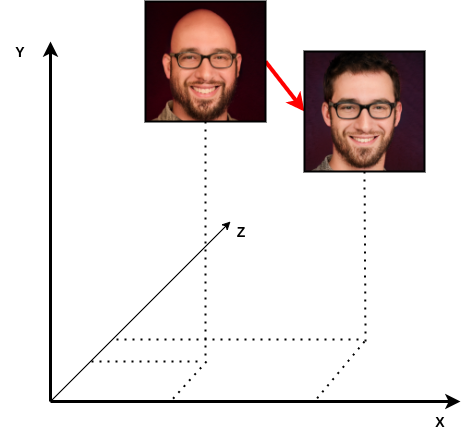
\includegraphics[width=0.5\textwidth]{images/feature-dir.png}
    \caption{Illustration of feature directions in latent space}
    \label{fig:feature_dir}
\end{figure}

Figure \ref{fig:feature_dir} further illustrates the idea of feature directions in the latent space. Here, we plot two face images in a $3D$ latent space. We can see that the difference between the two images in the existence and the absence of the hair, thus the red arrow represents the \emph{baldness} feature direction in that $3D$ latent space (moving along this particular vector causes hair density to change).

Our method of extracting the feature directions (\emph{hyperplanes}) consists of $3$ steps :
\begin{enumerate}
    \item \textbf{Code-Image Pairs Generation and Classification :} First, we use \texttt{StyleGAN2} to generate a large number of synthetic faces from random latent vectors. After so, we cluster the synthetic images (along with their latent vectors) according to each feature. The clustering can be based on discrete categories (like \emph{hair color} or \emph{race}) or continuous values (like \emph{hair length} or \emph{nose size}). We randomize the synthetic images in each clustering process to have better generalization and to cope with potential generation noise. For classification and regression, we use one of three possible methods, which are \textbf{manual labelling}, \textbf{classical image processing techniques} and \textbf{neural networks}. Thus, the output of this process is different groups of synthetic images sharing common facial features, along with their latent vectors.
    
    \item \textbf{Feature Directions Fitting :} Now, we have a set of latent vectors (\texttt{X}) and their corresponding feature values (\texttt{Y}). It's required to find a set of feature directions that satisfies the mapping between feature vectors and values. This problem can be formulated as :
    \begin{equation}
        Y = A_f \cdot X
    \end{equation}
    Where $A_f$ is the axis (direction) of feature $f$. \\
    We can obtain the solution to this equation in a closed form. However, due to the noise in both generation and classification, along with the non-linear nature of the problem, we opt to use \emph{ML} methods, specifically \textbf{Logistic Regression} and \textbf{SVM}. Meanwhile, we cannot see any difference between both methods, as they yield almost the same results. \\
    Finally, the generated feature directions are normalized to unit vectors :
    \begin{equation}
        A_{unit} = \frac{A}{||A||}
    \end{equation}
    
    \item \textbf{Directions Orthogonalization :} Facial features entanglement is one of the most difficult challenged of face generation. Some attributes in the human face tend to be extremely entangled by nature. For example, Asians rarely have curly hair, a woman cannot have beard and a man cannot put on makeup. Since \texttt{StyleGAN2} is trained and tuned on \textbf{FFHQ} dataset \cite{karras2019stylebased}, which contains real human faces, it is normal to notice some entanglement between some features. Consequently, the feature directions have to be further disentangled by using \emph{orthogonalization}. The orthogonalization process is done iteratively, starting from the most accurate feature directions. We orthogonalize other feature directions on the accurate ones, so that we have completely independent feature directions, where tuning one direction doesn't affect the others. The directions are orthogonalized as follows :
    \begin{equation}
        A_{proj} = (A \cdot B_{unit}) B_{unit}
    \end{equation}
    \begin{equation}
        A_{orthogonal} = A - A_{proj}
    \end{equation}
    To ensure convergence to reasonable set of feature directions, we use a threshold margin to stop the orthogonalization process, which is from $85$ to $90$ degrees ($5$ degrees on each side of normal angle).
\end{enumerate}

\paragraph{Initial Seed Generation}

\paragraph{Latent Manipulation}

\subsubsection{Design Constraints}

\subsubsection{Other Description}
